\documentclass[10pt,twocolumn]{article}
\usepackage[margin=2.3cm]{geometry}
\usepackage{float}
\restylefloat{table}
\usepackage{cite}
\usepackage{hyperref}
\usepackage{graphicx}
\usepackage{authblk}
\usepackage[latin1]{inputenc}
\usepackage{subfigure}
\usepackage{listings}
\usepackage{float}
\usepackage{fancyvrb}
\usepackage{multirow}
\usepackage{changebar}
%\usepackage{url}
\usepackage{array}
\usepackage{color}
\usepackage{rotating}
\usepackage{titlesec}
\restylefloat{figure}
\usepackage{epstopdf}
\usepackage{colortbl}
\usepackage{setspace}
%\usepackage{breakurl}
\usepackage[belowskip=-5pt]{caption}
\singlespacing
\input{macros}

\begin{document}
\title{{\bf Optimizing Latency and Throughput Trade-offs in a Stream Processing System}}
\author[1]{{Joao Carreira, Jian Neng Li}}
%\date{October 2014}
\date{}
\maketitle

%%%%%%%%%%%%%%%%%%%%%%%%%%%%%%%%%%%%%%%%%%%%%%
\begin{abstract}
\noindent The value of streaming systems such as Spark Streaming and Storm is derived from the timeliness of results. Less time to provide results means faster reaction. Nowadays, different streaming systems provide different end-to-end time guarantees, and these guarantees are to a large extent a result of each systems architecture. Spark Streaming is built on top of a general batch-processing framework to compute over mini-batches of streaming data. Storm allows the construction of topologies on which data flows to be processed. Spark Streaming is known to provide latencies on the order of seconds while Storm on the order of a few milliseconds. In this paper we investigate the approach taken by Spark Streaming and show that despite its more general architecture (\joao{general architecture may not be the right term}) it can provide latencies below 100ms. In this paper we make three contributions. First, we provide a comprehensive analysis of the performance of Spark Streaming and show where time is spent within the system. Second, we identify the performance and scalability bottlenecks of Spark Streaming and pinpoint the underlying architectural deficiencies of the system. Last, we propose three optimizations to reduce the system overhead and make it support higher levels of throughput.
        
%        To do so, we tackled two problems. The first has to do with overheads related to launching tasks and communicating between nodes. The second has to do with the poor scalability performance when the Spark is subject to a high number of tasks being scheduled. We show that with these two contributions Spark Streaming can support low-latency tasks and scale to demanding low-latency stream workloads.

%Large-scale data processing systems such as Spark and Hadoop MapReduce were developed for clusters built on commodity hardware. In this paper, we argue that current market trends invalidate some of the assumptions made by those systems, and we should therefore revisit the designs and architectures derived from them. For example, newer technologies including InfiniBand offer faster network connectivity, and advances in SSDs continue to drive down the cost of fast non-volatile memory. One new architecture that explores these new technologies is Firebox, a hardware building block for future Warehouse-Scale Computers (WSCs). We use Firebox in our studies, and evaluate the behavior changes of large-scale systems under the new settings. In particular, we measure the performance of Spark and applications in the Spark ecosystem under specific workloads, and critique the validity of its underlying assumptions and design decisions.

\end{abstract}

%\vfill
%\eject
%%%%%%%%%%%%%%%%%%%%%%%%%%%%%%%%%%%%%%%%%%%%%%
\section{Introduction}
Data analytics applications such as intrusion detection, web search and monitoring, require the computation of results in a timely fashion in order to provide interactivity and responsiveness. 
As enterprise workflows grow increasingly complex and applications become increasingly dependent on other applications, the latency guarantees of their processing systems become a major concern.
For instance, many systems today are designed to meet specific performance metrics or SLOs~\cite{Jockey}.
Applications that do not yield good performance may delay the execution of other systems and lead to loss of revenue and/or bad user experience.

Many data analytics 
systems~\cite{Millwheel,Babu:2001:CQO:603867.603884,TelegraphCQ,Storm,SparkStreaming,Trill,Naiad,Niagara,StreamInsight,Carney:2002:MSN:1287369.1287389,Sullivan:1998:TSM:1268256.1268258,condie2010mapreduce,Brito:2011:SLD:2114498.2116192, ELF} 
have been developed to provide easy-to-use and practical frameworks for stream processing, and they tend to follow one of the two popular approaches to act on inputs.
Systems like Storm or TelegraphCQ handle streams of data by creating pipelines for record-at-a-time processing. In this environment, data flows through the system (potentially through different machines) and is continuously processed and augmented.
Other systems like Spark Streaming and Trill rely on micro-batches. In these systems, records are coalesced into small groups before being processed together as batch jobs.

It is widely believed that to achieve low latency, applications should use the record-at-a-time approach, while for high throughput, the micro-batch model is more appropriate. 
The reason is that even though record-at-a-time systems can start processing data as soon as it is received, processing more records at a time will amortize the overheads associated with processing.
However, because records are not processed right away, the latency per record is higher on average.
In this paper, we are generally concerned with end-to-end latency, which the time between the application sending to data and the application receiving the output.

%However, these two approaches provide different trade-offs (as shown in table X).
The trade-offs between latency and throughput become less simple as applications are scaled out to run in a distributed fashion. In a distributed environment, the record-at-a-time approach has many disadvantages when compared with the micro-batch approach.
First, record-at-a-time systems are not suitable for stateful or blocking operators, as these operators by nature will unboundedly increase memory usage or stall the system. Although techniques such as punctuations~\cite{tucker2003exploiting} can be used, they place extra burden on the application. For micro-batch systems, because batches are of finite size, behaviors of stateful and blocking operators are much easier to define.
Second, record-at-a-time systems require replication or upstream backup techniques to tolerate failures. Neither of these solutions are desirable, because the former requires the usage of fail-over hardware, and the latter usually leads to high recovery times. When records are batched, fault tolerance can be implemented with methods such as backing up to a database~\cite{Storm} or keeping track of lineage information of batches~\cite{SparkStreaming}.
Finally, the programming model for micro-batch systems is very similar to that of a traditional batch system, making the process of developing streaming applications more familiar to developers.

Because of the advantages in the micro-batch model in distributed settings, we want to explore the possibilities of using this model to provide better end-to-end latencies. In this paper, we perform an in-depth analysis of Spark Streaming, a micro-batch streaming engine, and evaluate the system's ability to provide low-latency and high throughput stream processing.
In particular, we intend to answer the question: ``Are the performance limitations of Spark Streaming a consequence of its architecture, or the result of engineering decisions?"
Upon evaluating the system, our answer is: both. Although it is true that the percentage of the end-to-end latency spent in useful work is low, especially for small computations, some of the overheads can be reduced relatively easily. We focus on two such areas, task overheads and data storage speed, and present our results after the optimizations.

While the focus of our analysis is in Spark Streaming, we believe that our analysis and conclusions can inform the design and development of other streaming systems using the micro-batch architecture. The reason we chose Spark Streaming is that there is a fast-growing ecosystem of frameworks such as GraphX, MLlib, and SparkSQL being developed for Spark, the engine on top of which Spark Streaming is built. As a result, our work can potentially have large impact, since developers will be able to take advantage of both the rich tools as well as low end-to-end latency without sacrificing throughput.

The paper is organized as follows: 
in Section 2 we provide an overview of the architecture and workflow of Spark Streaming. 
In Section 3 we motivate this work with a performance study of Spark Streaming across two main dimensions: end-to-end latency and throughput.
In Section 4 we present optimizations aimed at solving some of the architectural deficiencies identified in the previous section.
In Section 5 we present some of the lessons gathered during this work and discuss some of the architectural changes we believe are required to make Spark Streaming provide lower latencies.
In Section 6 we describe how some other contributions relate and complement our work.
Finally, in Section 7 we summarize our research and discuss the next steps.



\section{Background}
% TODO:
% Why are we focusing on Spark Streaming?
%
To understand our work, we provide a short description of Spark Streaming's architecture.
\begin{figure}[t!]
  \begin{center}
    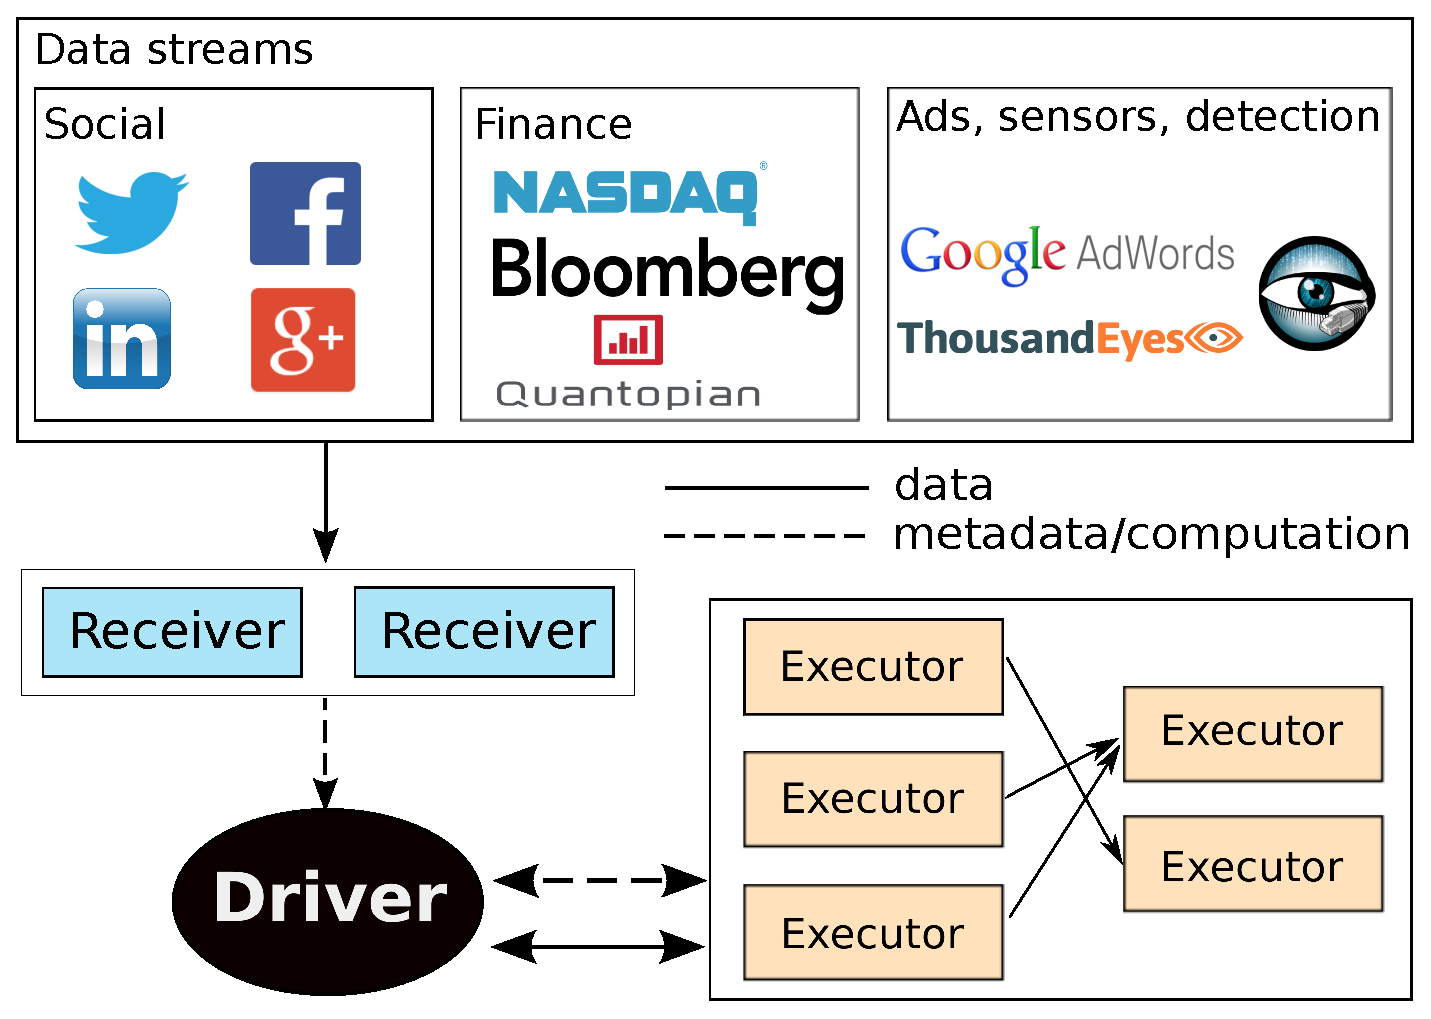
\includegraphics[scale=0.35]{images_graphs/spark_architecture_v4.eps}
  \end{center}
  \caption{Diagram of a Spark Streaming work flow. A Receiver and an Executor may execute in the same node.}
  \label{fig:SparkStreaming_architecture}
\end{figure}

Spark~\cite{Spark} is a general-purpose engine for large-scale cluster computing. It operates on Resilient Distributed Datasets (RDDs), an abstraction that represents read-only collections of objects partitioned across a set of machines. RDDs can be created from raw data or other RDDs. 
RDDs keep track of the bulk operations (e.g., map and reduce) performed on data (lineage) so that partitions can be recomputed if they are lost due to failures. 
Another feature of RDDs is that they can be persisted in memory, allowing efficient iterative computations.

Spark Streaming, the focus of our work, is a stream processing engine built on top of Spark.
It implements an abstraction called discretized streams (D-Streams), which takes advantage of RDDs to provide computations over windows of streaming records.
%which take advantage of RDDs to provide fast recovery after failures. 
The abstraction allows a micro-batch approach to streaming data, yielding high throughput, scalability and fault-tolerance.


The execution of a Spark Streaming job works as depicted in Figure~\ref{fig:SparkStreaming_architecture}. 
First, data is generated at a source (e.g., tweets from Twitter). As the data is generated, it is pushed to Spark Streaming, and is received by a Receiver. 
The Receiver is responsible for receiving input data and stash it in memory. Periodically, every \texttt{blockInterval} milliseconds, the Receiver takes the data stashed in memory and generates a block with it.
Once a block is generated, the Receiver informs a Spark Streaming's central component called Driver about this block. The Driver is responsible for holding metadata about the records received. 
Periodically, every \texttt{batchInterval} milliseconds, the Driver takes the blocks that have been communicated by the receivers and that have not been processed yet and generates a batch job. 
Once this batch job is generated it is appended to a queue of jobs to be scheduled. 
The scheduler continuously polls this queue and schedules the jobs in the machines available in the cluster.
Jobs are run in stateless isolated environments called Executors. Executors are usually deployed in the same nodes as Receivers.
Every batch job is divided into map and reduce stages, each of which contains tasks that need to be scheduled.

At the heart of the micro-batches approach taken by Spark is a trade-off between the amount of records Spark can process per unit of time and the time the system takes to return to the user the result of processing a stream record.
On one hand, waiting for more records to generate bigger batches allows Spark Streaming to amortize its overheads. On the other hand, the more time the system waits for data, the less responsive the system is.
Moreover, Spark can provide window semantics over data. For instance, a user can easily use Spark Streaming to compute the average temperature during the last 30 minutes over a stream of temperature sensor data.
%    This means that users can ask the system to compute 

%Internally, a variable called block interval controls the period of time before a receiver generates a new block. The total number of blocks generated in a batch interval corresponds to the number of tasks spawned for every stage of the resulting batch job.

Internally, Spark Streaming makes extensive use of Actors -- a design pattern that decouples the invocation of methods from their execution. 
In this approach, the invocation of methods between certain components is performed by inserting a message in a queue of the message receiver.
The component that receives the message continuously polls the queue and services messages in parallel.
This approach has been shown to provide high levels of concurrency and adaptability to changing loads~\cite{SEDA}.


\section{Motivation}
\begin{figure}[t!]
  \begin{center}
    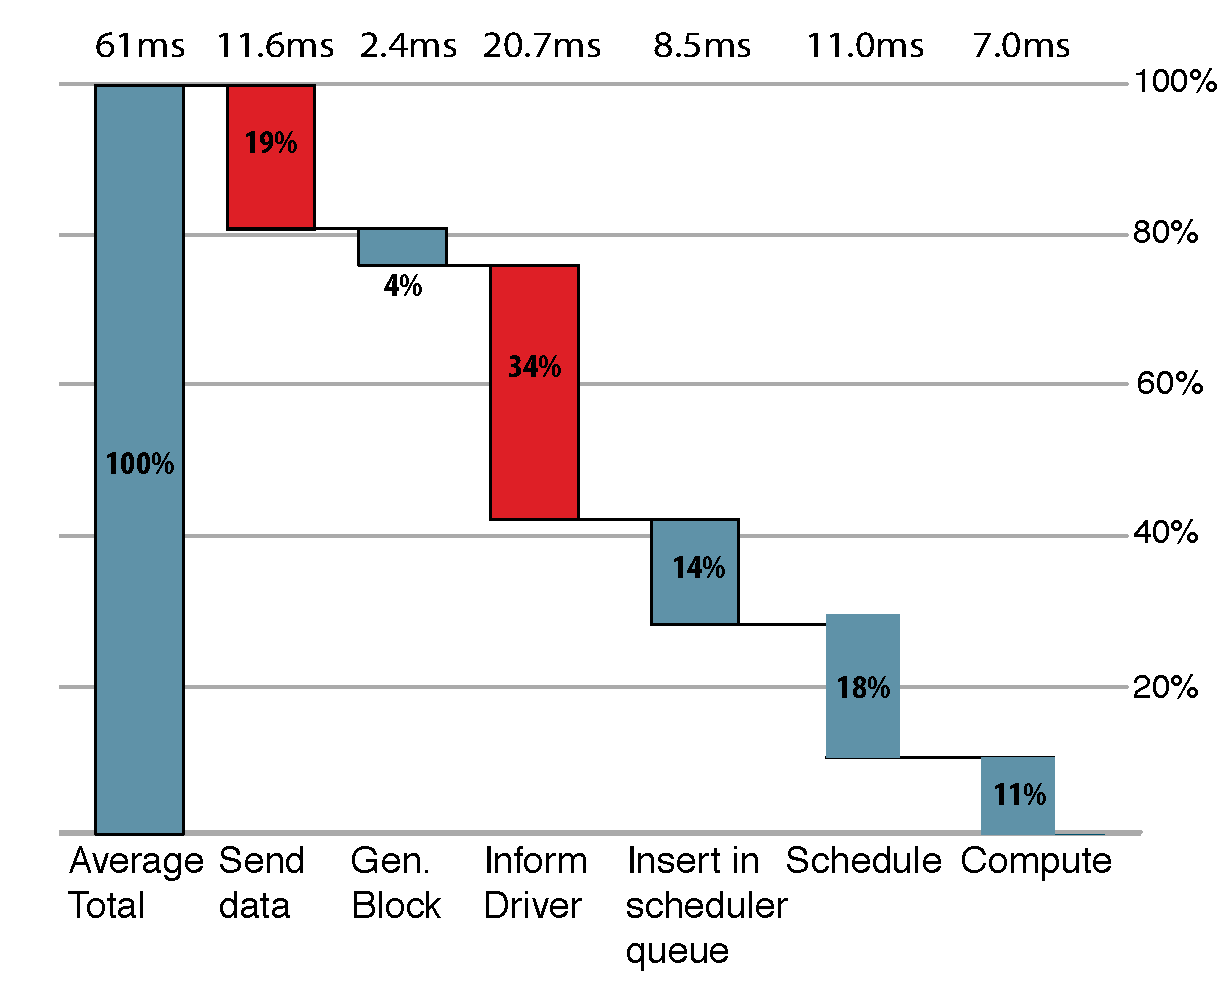
\includegraphics[scale=0.40]{images_graphs/waterfall/Rplots_illustrator.pdf}
  \end{center}
  \caption{}
  \label{fig:SparkStreaming_time_breakdown}
\end{figure}

To better understand the performance and limitations of Spark Streaming we conducted a benchmark study of the system.

To this end we have instrumented Spark Streaming.
Our instrumentation code allows us to track a subset of the stream data as it flows through the system.
We record at which moments of time some of the records pass through some of the components.

To exercise Spark Streaming we have used a synthetic workload.
%To this end we used a synthetic workload to exercise Spark Streaming and measure how the system behaves under different scenarios.
This workload consists of an application that listens for a stream of text records.
Each record has size between 15-25 bytes and holds a unique ID and a timestamp of time when the data was generated.
For each micro-batch, the application computes and records the end-to-end latency of the first 10 records in the micro-batch.

The computation performed by this workload is very lightweight.
We believe that this is in line with the type of computations used with Spark Streaming.
First, typical streaming tasks consist of filtering and/or simple aggregations.
These are operations that scale linearly with the amount of data in each batch.
Secondly, there is extensive work on optimizing the performance of query processing, both in batch and streaming contexts.
Finally, many steps of the computations performed in Spark and Spark Streaming are embarrassingly parallel. 
This means that developers can make use of more hardware to get better performance. 

%This is because first, the computation time is almost always orthogonal to the architecture used.
%Secondly, there is other work aimed at improving computation times in streaming or MapReduce systems.
%    There is parallel work on improving the performance of streaming computations that can be used to improve the execution times of tasks.

To run this benchmark, we have deployed a Receiver and a record generator in two different machines in the same cluster.

The record generator generates as many records as necessary to achieve a user-specified throughput.
Each record contains a timestamp that corresponds to the moment of creation of the record as well as a unique ID.
The Receiver uses the Spark Streaming API to consume this data. 
A task is generated periodically, according to a user-defined frequency, and scheduled to a node where the data is processed.

\begin{figure}[t!]
  \begin{center}
    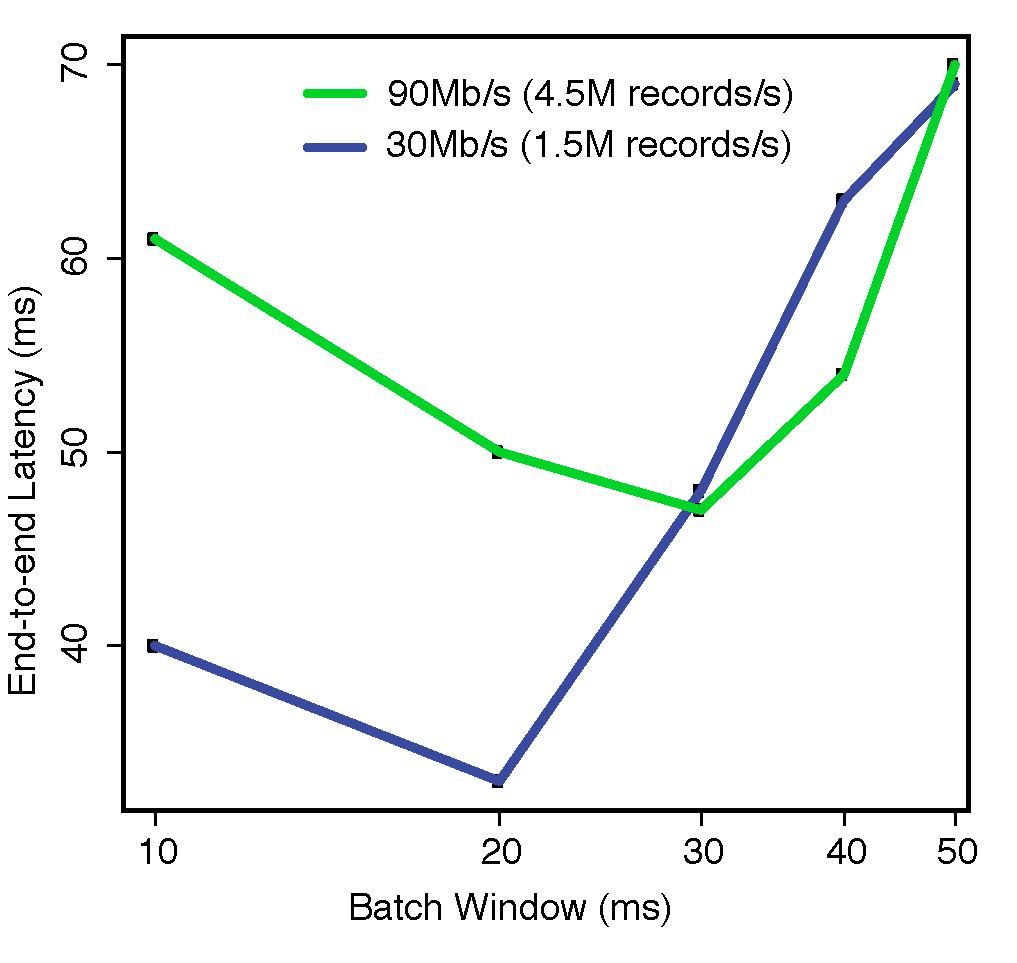
\includegraphics[scale=0.35]{images_graphs/batchsize_vs_latency/batchsize_vs_latency_illustrator.pdf}
  \end{center}
  \caption{\joao{Maybe put the legend inside the graph so the graph can be larger?}}
  \label{fig:Batchsize_vs_latency}
\end{figure}

We have instrumented the code of Spark Streaming to record the time at which the record transitions a phase (e.g., a task to process a record is scheduled).
%#understand how much time each record stays on each phase of the streaming process.
This allows us to gather 1) the time each record spends on each phase of the streaming process, and 2) the time between the generation of each record and the moment of computation -- end-to-end latency.

%When processing records, the time between the generation of each record and the moment of computation is captured. 
%We refer to this value throughout the paper as the end-to-end latency. 

The results of the first experiment we conducted are captured in Figure~\ref{fig:Batchsize_vs_latency}.
In this graph we show the average end-to-end latency obtained when running Spark Streaming with different batch windows and throughputs. 
Changing the batch window configuration allows us to tune the responsiveness of the system;
a lower value means that each records spends less time in memory waiting for a task to be spawned in order to process that same record. 
Varying the number of records generated by the stream source (throughput), allows us to understand how 
Spark behaves when it has to do more/less work per unit of time and how that affects latency.

As expected, as we instruct Spark Streaming to spawn tasks more frequently -- smaller batch window -- the average end-to-end latency time decreases.
However, at some point decreasing the batch window has a pernicious effect on the resulting latency.
Moreover, as we increase the throughput the end-to-end latency increases.
We have found that the Spark Streaming's Receiver can be a source of slowdown.
For instance, it is not able to receive more than roughly 30 MB/s (1.5M records).
This has to do with the fact that this component synchronously receives and stores streaming data. 


\section{Implementation}
The majority of the time processing a record is spent in the Receiver and during computation. 
In our experiments, we found that the rate at which the receiver can receive input is limited by the efficiency of the communication layer.
%does not increase significantly even if it drops every record.
Therefore, we did not treat this bottleneck as a problem fundamental within the architecture, and focused on scheduling and computation in our optimizations.

%\subsection{Scheduling Scalability}

%A significant amount of work has been done on scheduling. Many contributions aim to develop schedulers that can provide guarantees like fairness or utilization of resources~\cite{}. Others focus on making the schedule scale and/or provide low-latency scheduling of tasks~\cite{Sparrow, CFS}.
%
%During the execution of a Spark Streaming application, the Driver (a central component of Spark) generates tasks periodically and adds them to the tail of a scheduling queue. This queue is continuously probed by the scheduler, which schedules by taking tasks from the queue and sending them to worker nodes for processing.
%As applications specify lower batch intervals to process results more quickly, the number of tasks added to the queue per unit of time increases. Eventually, the scheduler will be unable to keep up with the rate of tasks being added to the queue. This results in an indefinite increase in the average time to schedule a task, which is worse considering the fact that tasks in one batch have less time to be processed before the next batch is generated.
%From this observation, we can see that lower batch intervals lead to lower task latencies, less throughput and more tasks scheduled per second. On the other hand, larger batch intervals lead to higher throughput, higher task latencies and less tasks scheduled per second. 
%
%To understand the performance of the current version of Spark Streaming, we have benchmarked the end-to-end latencies of tasks with different batch intervals. 
%Our benchmarks were run on a 16-node cluster, with each node having 16 cores. We have used 120 receivers on 4 nodes. 
%With this configuration, Spark Streaming generates 120$*$1000/(batch interval) tasks per second.
%Because we are solely interested in benchmarking the scheduling performance, we ran applications that generate no-op tasks.
%
%We have found that for a batch interval less than 40ms the system becomes unstable because the scheduler cannot keep up with the rate of tasks generated. This instability leads to increasingly higher scheduling delays and increasing garbage collection activity due to higher memory usage. \joao{Need a graph here showing end-to-end latency of tasks with varying batch intervals}

%To enable a higher scheduling rate of tasks by Spark Streaming, we propose to 1) schedule all tasks per worker in bulk and 2) physically decouple the scheduling (Scheduler) of tasks from their generation (Driver).
%First, at each scheduling stage, instead of sending multiple tasks for each node separately, we coalesce them into the same message. This reduces the serialization and networking overheads that result from sending many small messages.
%Secondly, as the task generation rate surpasses the scheduling rate, the driver elastically spawns schedulers in remote physical nodes. Thereafter, tasks are forwarded, according to some policy, to these newly spawned schedulers for scheduling (see Figure \ref{fig:schedarch}). 
%
%We have implemented this decentralized architecture in Spark Streaming. Due to the instability of connections between the schedulers, the driver and the workers -- connections are dropped after running the system for a few minutes -- we are currently not able to evaluate the performance benefits of this technique. We plan to fix this engineering problem and report on further results.
%
%\subsection{Task overheads}

Since our synthetic benchmark performed trivial computation, most of the time spent in the ``computation" part of the graph should be due to the overheads in launching and running tasks. 

To breakdown the process of running desks, we modified the receiver so that it generated a block regardless of the number of records received. We then ran the system on empty input, using an application that required a single stage. Since there was no input, the computation itself was effectively no-op. After profiling this workflow, we found that from the driver's perspective, the time it took for a task to be scheduled to the time it took for the result to be received was around 5.0ms. However, approximately 3.6ms out of this time was spent deserializing the task. These numbers suggest that if we can reduce the task deserialization time, there will be a considerable improvement to the latency of small tasks.

\begin{figure}[t!]
 \begin{center}
   \includegraphics[scale=0.30]{images_graphs/deserialization.eps}
 \end{center}
 \caption{How a task is deserialized on the executor. Examples of new dependencies can be new libraries needed to run the current task.}
 \label{fig:deserialization}
\end{figure}

Having discovered that a significant portion of the time running small tasks is spent in deserialization, we further measured the time it took for individual components of deserialization to complete. Figure \ref{fig:deserialization} summarizes the process of task deserialization on the executor. An array of bytes called \texttt{serializedTask} is deserialized into a tuple of \texttt{taskFiles}, \texttt{taskJars}, and \texttt{taskBytes}, the first two of which are passed into a method called \texttt{updateDependencies()}, while the latter is further deserialized into a \texttt{Task} object. The \texttt{Task} object contains information such as the function to run, the RDD to use, and the partition of the RDD to operate on.

\begin{figure}[t!]
 \begin{center}
   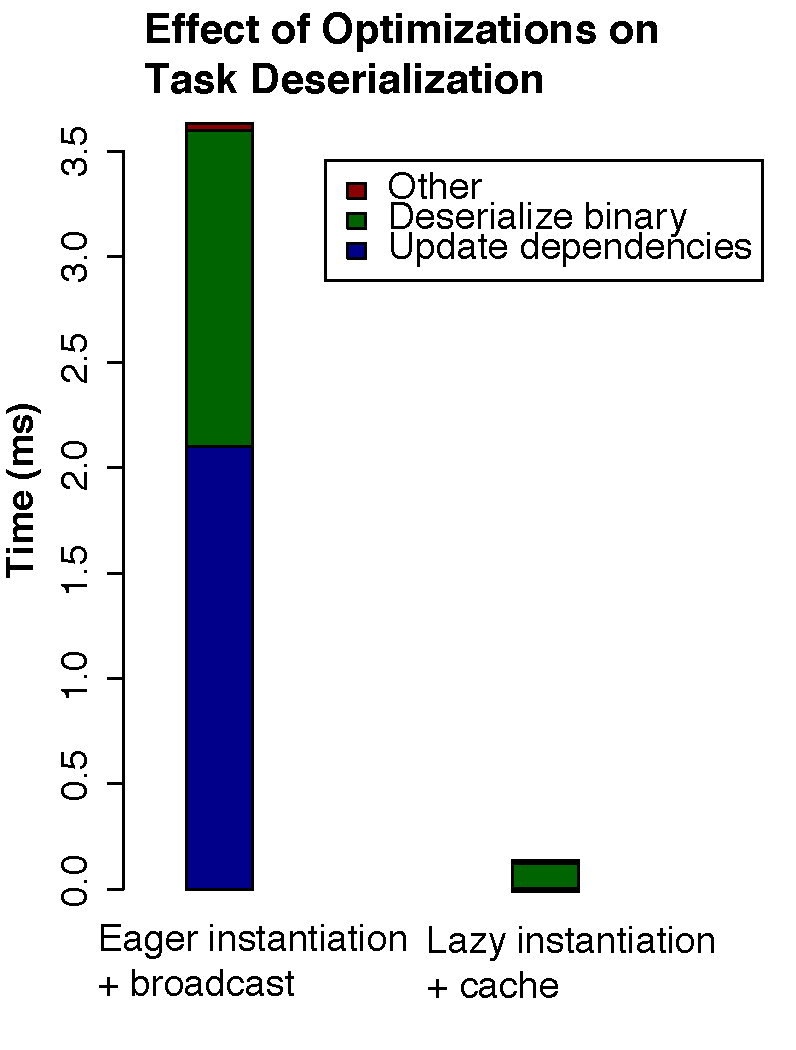
\includegraphics[scale=0.60]{images_graphs/optimizations/graph2/task_deser_micro.pdf}
 \end{center}
 \caption{Breakdown of average time spent deserializing a task before and after adding lazy instantiation of configuration object and caching task binaries.}
 \label{fig:deserialization_times}
\end{figure}

Figure \ref{fig:deserialization_times} shows a time breakdown of deserialization. As can be seen in the graph, majority of the time in this case are in updating dependencies and deserializing \texttt{taskBytes}. We next examine each of these two components in more detail.

\subsubsection{Deserialize Binary}
In order to reduce the amount of duplicate data transferred, Spark 1.1.0 wraps the function and the RDD into a broadcast variable. This way, each executor will only fetch the function and the RDD of a batch once. The first task that uses the information will pull it from the driver, and cache the result within the executor for later tasks. In the Spark Streaming context however, this means for every stage, some task on every executor requires a round trip to the driver to fetch the broadcast variable, increasing the latency. As the batch interval shrinks, new RDDs are created more often, but the functions to operate on them do not change. The executor should be able to cache them for a longer period of time than only for the current stage.

To eliminate this round trip, we experimented with caching of \texttt{taskBytes}. The cache is implemented by keeping track of previously broadcasted \texttt{taskBytes} on the driver, and refer to their IDs instead of creating a new broadcast variable every time. Broadcast variables are automatically cached on the executor side, so this this methodology removes the extraneous communication with the driver.

\subsection{Update Dependencies}
In \texttt{updateDependencies()}, the current implementation creates a new Hadoop configuration object regardless of whether new dependencies are introduced. However, this objection creation is very costly in CPU cycles. Moreover, since a streaming application rarely introduces new dependencies once it starts to run, this method is incurring unnecessary costs. To solve this problem, we changed the object to be lazily instantiated, so that no cycles are spent creating the configuration object unless new dependencies are introduced.

\subsection{Evaluation}
The improvements of the two optimizations described above are also shown in Figure \ref{fig:deserialization_times}. After the changes, deserialization time for a task decreased from 3.6ms to 0.2ms. The impact of the two changes on overall task runtime is reflected in Figure~\ref{fig:runtime_optimizations}.

\begin{figure}[t!]
 \begin{center}
   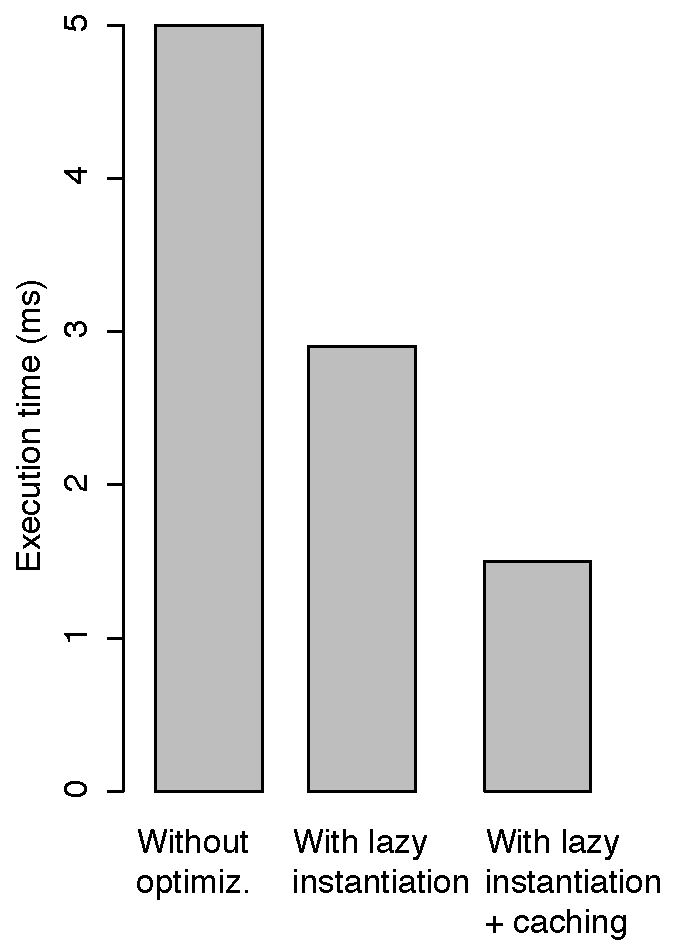
\includegraphics[scale=0.60]{images_graphs/optimizations/graph3/runtime_optimizations.pdf}
 \end{center}
 \caption{Average time spent in running no-op tasks before and after the optimizations in deserialization.}
 \label{fig:runtime_optimizations}
\end{figure}

To show the effect of reducing task runtimes, we performed a micro-benchmark running a single stage with many tasks. The results are shown in Figure \ref{fig:lazy_micro}

\begin{figure}[t!]
 \begin{center}
   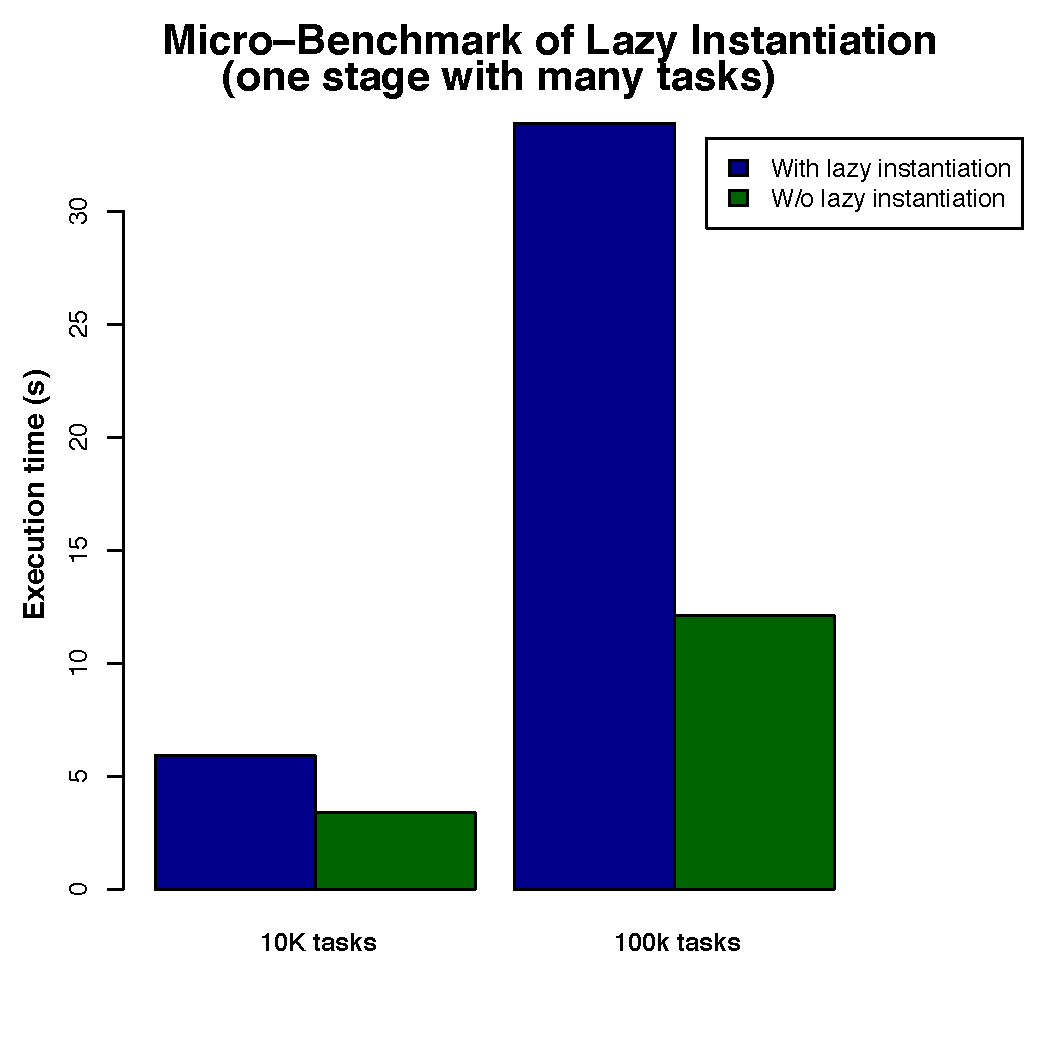
\includegraphics[scale=0.50]{images_graphs/optimizations/graph1/lazy_micro.pdf}
 \end{center}
 \caption{Amount of time spent running a single Spark stage consisting of many tasks without and with lazy instantiation of configuration object.}
 \label{fig:lazy_micro}
\end{figure}

\subsection{Limitations}
While caching task binaries sound simple in theory, they are more complicated to implement in practice. For example, in our implementation, the Driver caches the serialized binary of tasks. For serializations across batches to match, we made fields such as IDs that are unique across objects not be serialized. While this change does not affect correctness, it will complicate other components such as logging that uses those information.

Furthermore, our caching technique only works for batches with single stages. When there are multiple stages, i.e. when shuffles or aggregations are involved, the dependency in previous data tends to change from batch to batch, making it difficult to hit a previously cached binary.


\section{Lessons and Discussion}
Having conducted various benchmarks of Spark Streaming for this research, we have found various parameters that can be used to tune the performance of the system. These parameters include the number of Receivers, the batch window size, the size of input records, and whether the input data is serialized. In this section we will describe in detail about their impacts on the end-to-end latency or throughput. We believe these parameters reflect configuration parameters common to micro-batch streaming systems and thus these lessons are generally applicable.

\paragraph{Number of Receivers}
In our synthetic benchmark using 20-byte records, a single Receiver is able to take in at most around 30MB/s, or 1.5M records/s, even after we modified the code to immediate drop instead of storing the data. While the throughput does not seem very high, 1.5M records is 2.5 times the 600K records per second per node recorded by the original Spark Streaming paper. This insight tells us that when evaluating throughput of a system, both the volume of data as well as the size of input data should be taken into consideration.

To overcome the bottleneck in data intake, the solution can be as simple as increasing the number of Receivers. It is also possible to obtain the performance gain by setting the number of Receivers larger than the number of physical machines.

\paragraph{Size and Number of Input Records}
As explained by the previous subsection, the size and number of input records affect the system's performance in terms of throughput. As the size of the records increases, the throughput of the system in volume will also increase linearly to a point, since more data is processed per record. Conversely, as the size of input decreases, the Receiver eventually reaches a bottleneck in the number of records that it can handle (around 1.5M/s).

\paragraph{Size of Batch Interval}
While the micro-batch approach increases throughput at the expense of latency by coalescing input data before processing, the size of the batch interval does not form a linear relationship with the throughput. In fact, the best latency is obtained when the batch interval is set to slightly larger than the time it takes to computationally process a batch. This difference accounts for overheads in task spawning, scheduling, and noise. In practice, instead of using trial and error, it would be best if the system can dynamically adjust the duration of the batch interval based on inputs. Dynamic batch sizes in addition will have the ability to adjust to sudden changes in data incoming rates.

\paragraph{Input Serialization}
In Section 3, we evaluated the system using plain text input records. However, in real world applications, applications may choose to serialize their input data for better network latency. Serializing input data means they have to be deserialized during computation, so this decision concerns the trade-off between CPU and network I/O.

In the case of Spark Streaming, if the input data is serialized, it has the option to be directly stored inside the system as a block, bypassing the block interval and logic to convert stored records into blocks. Not surprisingly, this approach increases the rate at which Spark Streaming can intake data significantly. For the same benchmark with 20-byte records, Spark Streaming can sustain a throughput of 80MB/s, or 16M records per second using a single Receiver.

The disadvantage of sending data directly as blocks is that they need to be coalesced at the application, i.e. the application needs to group input records together and send them as a block to Spark Streaming. This number should be relatively large: when Spark Stream receives blocks only containing single records, its throughput dropped to around 375KB/s, or 75K records/s.

%In this section we show that Spark Streaming is able to provide low end-to-end batch response times for a realistic and demanding workload. We also show that our contributions decrease the average batch latency by Y times and increases the scalability of the system from X tasks/s to Y tasks/s.

%In order to evaluate our contributions we have setup an instance of Spark Streaming to process a stream of tweets from Twitter. In our setup Spark Streaming runs in a dedicated cluster of 16 nodes. Each node has 16 cores  Intel IvyBridge 3.0GHz with 64GB of RAM. The nodes are interconnected with InfiniBand connections. We ran this experiment with 1 driver, 15 workers and X receivers.

%\paragraph {\bf Twitter Workload} To approximate as much as possible a real workload we have built a custom twitter receiver. This receiver listens for tweets using the standard Twitter API. Because this API samples the tweets (roughly 1\% of the tweets are published), every time we receive tweets from this 

%\paragraph{Producers, Consumers, and Queues}
%As we have found through our initial benchmark in Section 3, when the batch interval becomes shorter than the optimal, the end-to-end latency increases dramatically. From the average time break down shown in Figure~\ref{fig:Batchsize_vs_latency}, we can see a significant portion of the latency is spent receiving the data as well as sending the generated block to the Driver. What these two components share in common is that the data and metadata being moved around follow the producer/consumer pattern, with a queue acting as the middleman. As either side becomes overwhelmed, the size of the queue becomes larger, and latency increases. This architecture stems from SEDA~\cite{SEDA}, which was proposed as a way to serve web requests in multiple event queues. An interesting future work in this area would be to apply similar optimizations as have been done to SEDA, and compare the results.

\paragraph{Others} There are also a number of areas which we did not explore, either due to time or resource constraints. First, likely due to the reason that we only had access to 16 machines, scheduling and network communication were never bottlenecks. Second, as we are targeting very low latency streaming workloads, we did not benchmark in detail the performance of the system running applications that involve shuffles and aggregations, i.e. multiple stages per batch. Finally, we did not look into the implications of low latency in the Spark Streaming architecture when fault tolerance becomes a concern.


\section{Related Work}
\paragraph {\bf High Throughput} Trill~\cite{Trill} is a recent query processor for analytics that uses a tempo-relational model, enabling it to support a wide range of latencies for both online and offline data. It achieves high performance by using a streaming batched-columnar data representation, to provide data locality and reduce data access time.
The original Spark Streaming~\cite{SparkStreaming} paper placed emphasis on fault-tolerance, straggler mitigation, fast recovery, and scalability, in the context of high throughput. Our work builds on top of this belief in high throughput, without removing any of the features in the system.

\paragraph {\bf Adaptive Batch Sizes} TelegraphCQ~\cite{TelegraphCQ} is a system designed for a volatile environment, and can make per-tuple and per-operator routing decisions to balance load. \cite{das2014adaptive} studies the effect of batch sizes and other parameters on the throughput and end-to-end latency of the system, and proposes an algorithm based on Fixed-Point Iteration to automatically adapt batch sizes as the circumstance varies. Although there is currently no such mechanism implemented in Spark Streaming, adaptive batch sizes can be very useful in determining the right value for the best trade-offs.

\paragraph {\bf Low Latency} Some past work has focused on reducing the time to show results. Systems like BlinkDB~\cite{BlinkDB} perform computations on samples of the data and return prematurely with error bars, while ideas like online aggregation~\cite{OnlineAggregation} show current results as the query goes to completion.
While we did not sample data in our research, we see these techniques as complementary to our work, as they can be used to reduce the overall time of streaming computations.
Others systems such as Incoop~\cite{Incoop} perform computation incrementally in order to avoid repeating previous computations. Storm~\cite{Storm} also a real-time, fault-tolerant distributed stream processing system that allows record-at-a-time approach for low latency.

\paragraph {\bf Scheduling} Extensive research has been done on how to improve the scheduling of tasks in MapReduce frameworks. 
Systems like Sparrow~\cite{Sparrow} focus specifically on scenarios where the number of tasks to be scheduled is very large.
Even though we haven't identified the scheduler of Spark Streaming as an immediate bottleneck, we believe that methods like decentralized scheduling can be useful. As tasks become shorter, the scheduler may be forced to schedule more tasks per unit of time. 


\section{Conclusion and Future Work}
This paper presents an analysis of low-latency stream processing in Spark Streaming, a space that we have found this system lacking in practice.
We make three contributions to achieve this goal: 1) analysis of Spark Streaming performance, 2) identification of main bottlenecks in the system, and 3) design and evaluation optimizations to reduce overheads.

Much of this work is still in progress. We plan to continue working on this problem and evaluating the solutions we have proposed. 


%%%%%%%%%%%%%%%%%%%%%%%%%%%%%%%%%%%%%%%%%%%%%%%%%%%%%%%%%%%%%%%%%%%%%%%%%%%%%%%%
% \pagebreak
\bibliography{main}
\bibliographystyle{abbrv}

\end{document}
